\section{Customizing Look}
\subsection{Annotations}
To emphasize some parts of the network topology, you can add various graphic
elements to the canvas. These elements are divided into three groups:
\begin{itemize}
    \item Text
    \item Freeform
    \item Oval
    \item Rectangle
\end{itemize}
Each of these elements have their own tools in the toolbox: \emph{Text} tool
(Figure \ref{fig:text}), \emph{Freeform} tool (Figure \ref{fig:freeform}),
\emph{Oval} tool (Figure \ref{fig:oval}) and \emph{Rectangle} tool (Figure
\ref{fig:rectangle}).

\begin{figure}[H]
  \centering
  \vspace{10pt}
  
\includegraphics[width=0.07\textwidth]{./images/text_tool.png}
  \caption{\emph{Text tool}}
  \label{fig:text}
\end{figure}

\begin{figure}[H]
  \centering
  \vspace{10pt}
  
\includegraphics[width=0.07\textwidth]{./images/freeform_tool.png}
  \caption{\emph{Freeform tool}}
  \label{fig:freeform}
\end{figure}

\begin{figure}[H]
  \centering
  \vspace{10pt}
  
\includegraphics[width=0.07\textwidth]{./images/oval_tool.png}
  \caption{\emph{Oval tool}}
  \label{fig:oval}
\end{figure}

\begin{figure}[H]
  \centering
  \vspace{10pt}
  
\includegraphics[width=0.07\textwidth]{./images/rectangle_tool.png}
  \caption{\emph{Rectangle tool}}
  \label{fig:rectangle}
\end{figure}

To add an annotation to the canvas, select the appropriate tool and click (and
drag) where you want to add the annotation. A popup window will be shown. There
you can define how will the annotation look.

When created, annotations can be moved around on the canvas. This is done by
using the select tool. Click on the annotation and then drag it to its
destination.

\subsubsection{Text}
The text annotation lets you define the following options(Figure
\ref{fig:text_conf}):
\begin{itemize}
    \item \emph{Text color} - color of the text in RGB values
    \item \emph{Font} - which system font, size and style you want to use
\end{itemize}

\begin{figure}[H]
	\centering
	\vspace{10pt}
	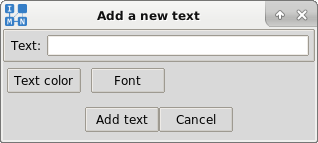
\includegraphics[width=0.55\textwidth]{./images/text_conf.png}
	\caption{\emph{Text configuration window}}
	\label{fig:text_conf}
\end{figure}

\subsubsection{Freeform}
The freeform configuration window includes:
\begin{itemize}
	\item \emph{Line color} - which line color to use
	\item \emph{Width} - line width to use
\end{itemize}

\begin{figure}[H]
	\centering
	\vspace{10pt}
	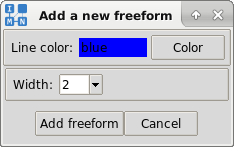
\includegraphics[width=0.30\textwidth]{./images/freeform_conf.png}
	\caption{\emph{Freeform configuration window}}
	\label{fig:freeform_conf}
\end{figure}

\subsubsection{Oval}
The size of the oval annotation is defined by dragging the cursor on the canvas
while keeping the left mouse button pressed. When the annotation size seems to
be fine, release the mouse button. The oval configuration window will popup
(Figure \ref{fig:oval_conf}).

The oval annotation lets you define the following additional options (Figure
\ref{fig:oval_conf}):
\begin{itemize}
    \item \emph{Fill color} - color of the annotation fill in RGB values.
    \item \emph{Border color} - color of the annotation border in RGB values.
    \item \emph{Border width} - width of the annotation border.
\end{itemize}

\begin{figure}[H]
	\centering
	\vspace{10pt}
	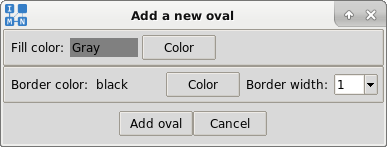
\includegraphics[width=0.55\textwidth]{./images/oval_conf.png}
	\caption{\emph{Oval configuration window}}
	\label{fig:oval_conf}
\end{figure}

\subsubsection{Rectangle}
The rectangle configuration window has the same options as the oval
configuration window. The rectangle size is defined the same way as the size of
the oval.

The rectangle annotation lets you define the following additional options
(Figure \ref{fig:rectangle_conf}):
\begin{itemize}
    \item \emph{Radius of the bend at the corners} - defines roundness of the
rectangle edges.
\end{itemize}

\begin{figure}[H]
	\centering
	\vspace{10pt}
	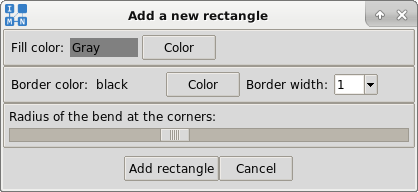
\includegraphics[width=0.55\textwidth]{./images/rectangle_conf.png}
	\caption{\emph{Rectangle configuration window}}
	\label{fig:rectangle_conf}
\end{figure}

Example of the annotations usage is shown in Figure \ref{fig:annotations_example}.

\begin{figure}[H]
	\centering
	\vspace{10pt}
	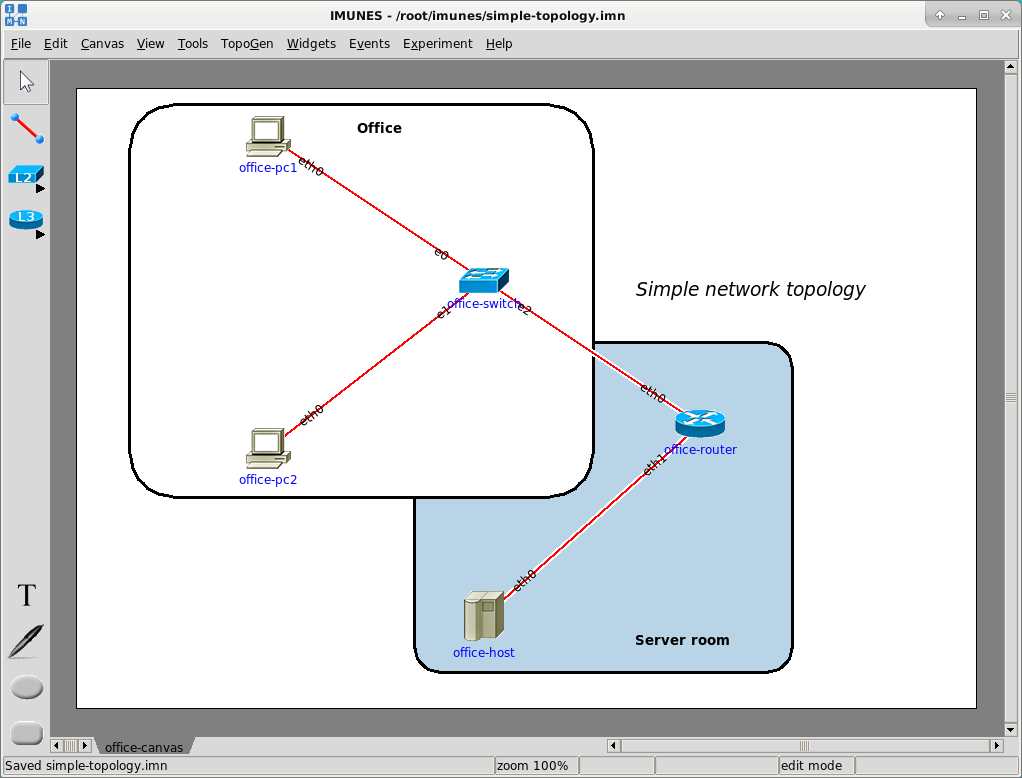
\includegraphics[width=\textwidth]{./images/annotations_example.png}
	\caption{\emph{Annotations example}}
	\label{fig:annotations_example}
\end{figure}

\subsection{Canvas background image}
\label{sec:CanvasBackgroundImage}

The options for changing the canvas background image are accessible through the
\emph{Canvas} and \emph{View} menu and through the menu that is opened with a
right click on the empty canvas (Figure \ref{fig:canvas_menu} and Figure
\ref{fig:background_image_menu}).

\begin{figure}[H]
	\centering
	\vspace{10pt}
	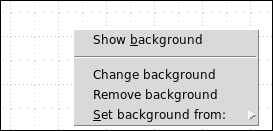
\includegraphics[width=0.4\textwidth]{./images/background_image_menu.png}
	\caption{\emph{Background image menu}}
	\label{fig:background_image_menu}
\end{figure}

All options related to the canvas background are accessible in the
\emph{Background image} menu (Figure \ref{fig:background_image_menu}):
\begin{itemize}
    \item \emph{Show background} - Show or hide the canvas background.
    \item \emph{Change background} - Opens the \emph{Change canvas background}
window (Figure \ref{fig:change_canvas_background}).
    \item \emph{Remove background} - Removes the background from the current
canvas.
    \item \emph{Set background from} - Sets the background from an another
canvas.
\end{itemize}

To set a canvas background you need to open the \emph{Change canvas background}
window (Figure \ref{fig:change_canvas_background}).

\begin{figure}[H]
	\centering
	\vspace{10pt}
	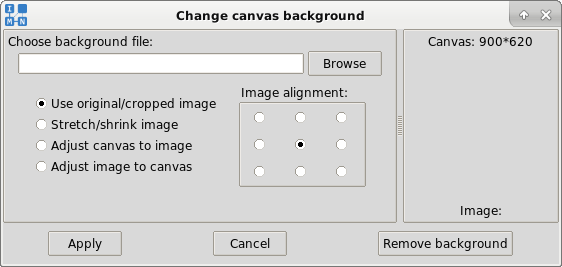
\includegraphics[width=0.75\textwidth]{./images/change_canvas_background.png}
	\caption{\emph{Change canvas background}}
	\label{fig:change_canvas_background}
\end{figure}

This window is divided into two main parts:
\begin{itemize}
    \item Left pane with the canvas background options
    \begin{itemize}
	\item Field and button for choosing the background image
	\item Image setting options
	\item Image alignment options
	\item Additional information if imagemagick is not present (Figure
\ref{fig:imagemagick_warning})
    \end{itemize}
    \item Right pane with canvas and image information and preview
    \begin{itemize}
	\item Canvas size information
	\item Image preview
	\item Image size information
    \end{itemize}
\end{itemize}

\begin{figure}[H]
	\centering
	\vspace{10pt}
	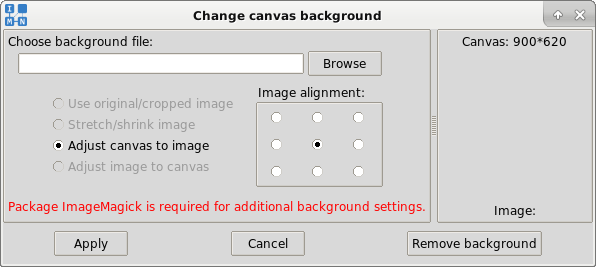
\includegraphics[width=0.78\textwidth]{./images/imagemagick_warning.png}
	\caption{\emph{Warning if ImageMagick is not present}}
	\label{fig:imagemagick_warning}
\end{figure}


When the image is selected there are four image setting modes that can be chosen:
\begin{itemize}
    \item \emph{Use original/cropped image} - If the image is smaller it will
be placed in the position defined by the image alignment. If the image is
larger  it will be cropped. The image alignment will define which part of the
image will be taken as the background.
    \item \emph{Stretch/shrink image} - If the image is smaller it will be
stretched without changing the proportions. If the image is larger it will be
shrunk without changing the proportions. The image alignment will define which
part of the image will be taken as the background.
    \item \emph{Adjust canvas to image} - The canvas will be resized to the
image size and then the background image will be set.
    \item \emph{Adjust image to canvas} - The image will be forcibly resized to
the canvas size with changed proportions if needed.
\end{itemize}

\subsubsection{Settings canvas background images}

We will use the extended topology example (\emph{extended-topology.imn}) to set
canvas background images. On the \emph{office-canvas} we will set a background
image. Then we will go to the \emph{roadwarrior-canvas} and set that same image
using the \emph{Set background from $\to$ office-canvas} option (Figure
\ref{fig:set_background_from}).

\begin{figure}[H]
	\centering
	\vspace{10pt}
	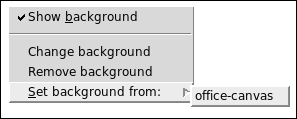
\includegraphics[width=0.4\textwidth]{./images/set_background_from.png}
	\caption{\emph{Set background from menu}}
	\label{fig:set_background_from}
\end{figure}

The final result is shown in Figure \ref{fig:canvas_background_example_1} and
Figure \ref{fig:canvas_background_example_2}.

\begin{figure}[H]
	\centering
% 	\vspace{10pt}
	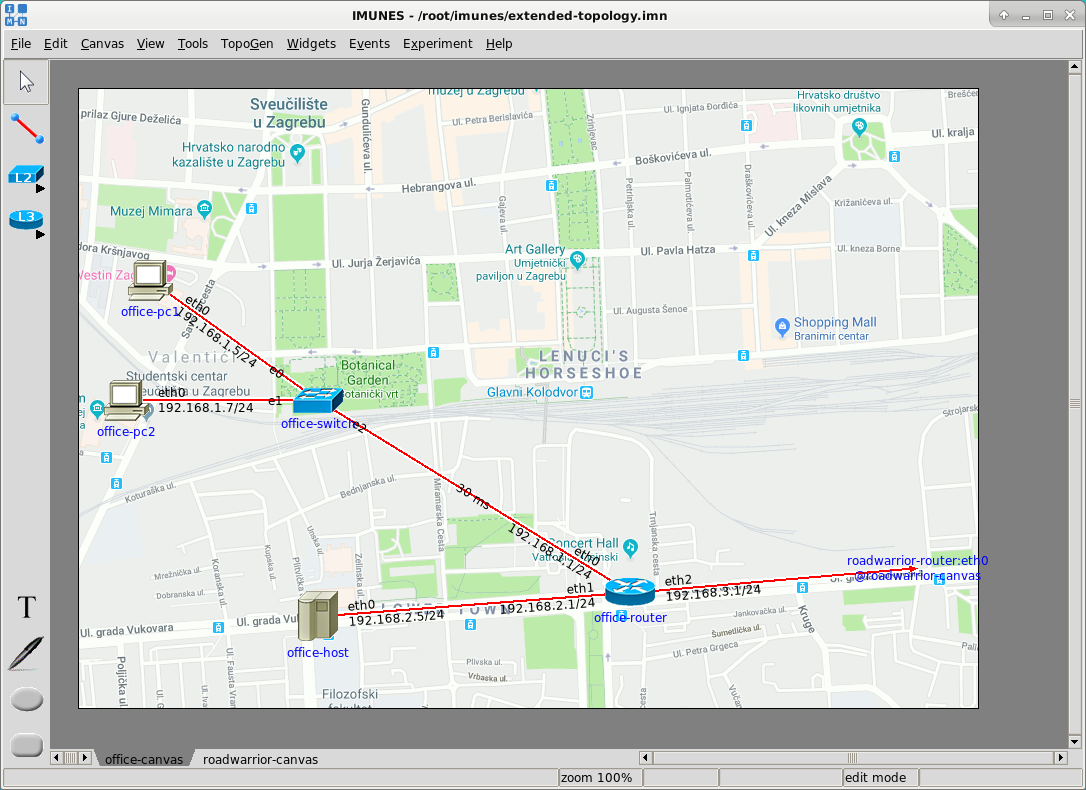
\includegraphics[width=\textwidth]{./images/canvas_background_example_1.png}
	\caption{\emph{Canvas background example on office-canvas}}
	\label{fig:canvas_background_example_1}
\end{figure}

\begin{figure}[H]
	\centering
% 	\vspace{10pt}
	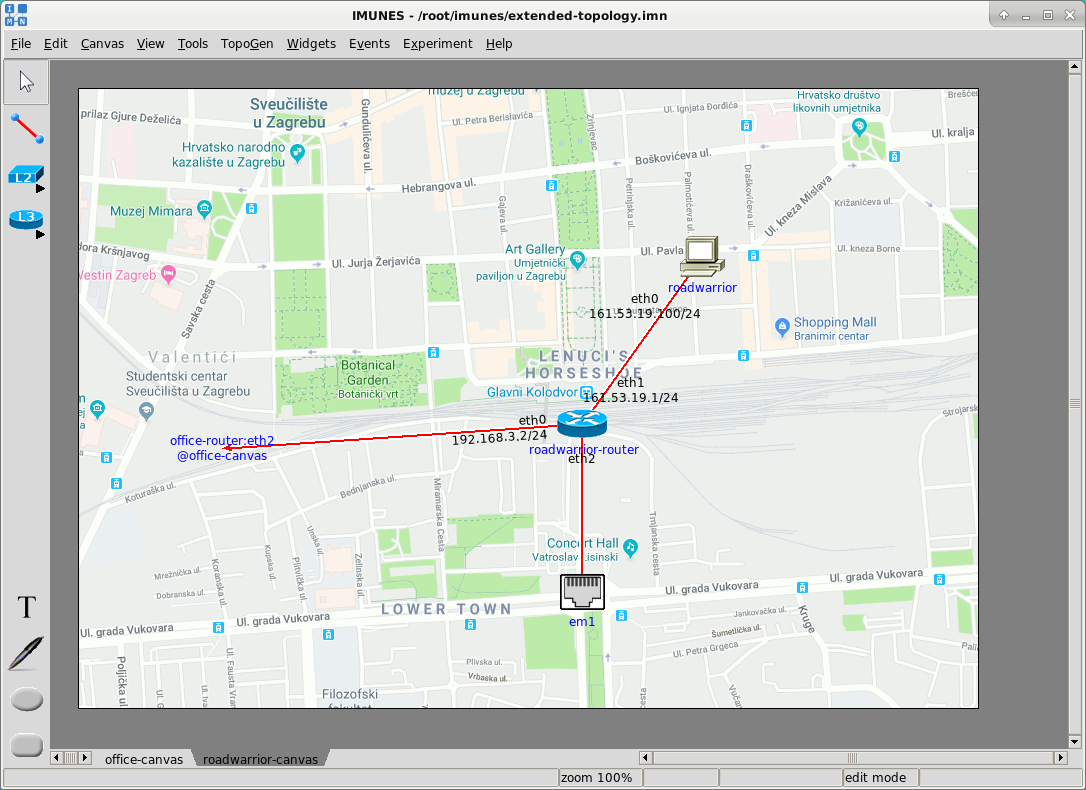
\includegraphics[width=\textwidth]{./images/canvas_background_example_2.png}
	\caption{\emph{Canvas background example on roadwarrior-canvas}}
	\label{fig:canvas_background_example_2}
\end{figure}

\subsection{Icons}
\label{sec:Icons}
IMUNES lets you choose custom node icons. First, select the nodes whose icons
you want to change. Then right click on the selection and then go to the
\emph{Node icon $\to$ Change node icons} option (Figure
\ref{fig:node_icon_menu}). This menu has also the \emph{Set default icons}
option that sets the default node icon for the selected icons.

\begin{figure}[H]
	\centering
	\vspace{10pt}
	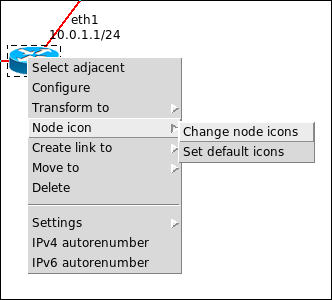
\includegraphics[width=0.5\textwidth]{./images/node_icon_menu.png}
	\caption{\emph{Node icon menu}}
	\label{fig:node_icon_menu}
\end{figure}

The \emph{Change node icons} option opens the \emph{Set custom icon} window
(Figure \ref{fig:set_custom_icon}).

\begin{figure}[H]
	\centering
	\vspace{10pt}
	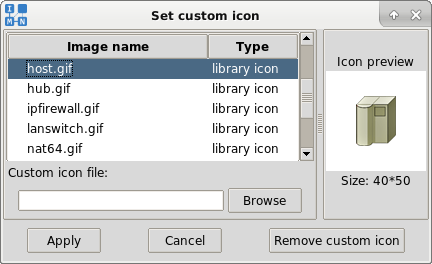
\includegraphics[width=0.6\textwidth]{./images/set_custom_icon.png}
	\caption{\emph{Set custom icon}}
	\label{fig:set_custom_icon}
\end{figure}

This window is divided into two main parts (Figure \ref{fig:set_custom_icon}):
\begin{itemize}
    \item Left pane for choosing custom icons
    \begin{itemize}
	\item List of library and custom icons on the top. Every icon that has
been used or is being used in the project will be available at the end of the
list, and will be given a generic name (e.g. img0, img5).
	\item Field and button for choosing the custom icon
    \end{itemize}
    \item Right pane with the icon preview and icon size information
\end{itemize}

We will now open the \emph{extended-topology.imn} file and set a custom icon.
We will choose the library icon \emph{ipfirewall.gif} for the
\emph{roadwarrior-router}. The final result is shown on Figure
\ref{fig:changed_node_icon}.

\begin{figure}[H]
	\centering
	\vspace{10pt}
	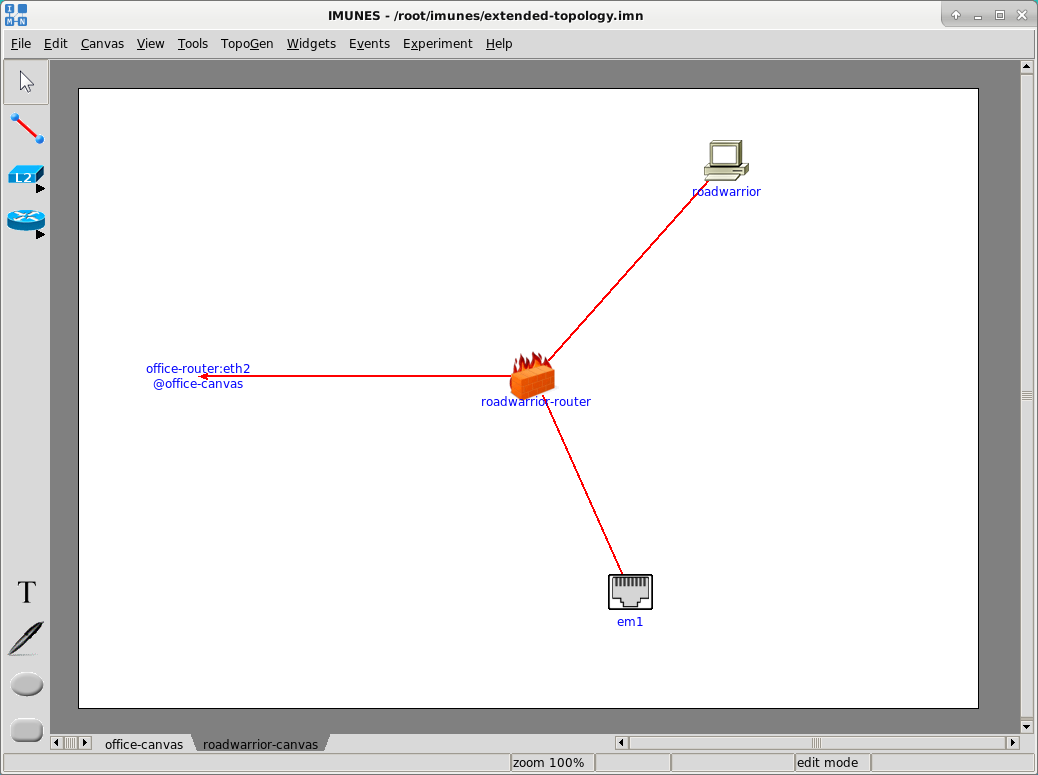
\includegraphics[width=\textwidth]{./images/changed_node_icon.png}
	\caption{\emph{Changed roadwarrior-router icon}}
	\label{fig:changed_node_icon}
\end{figure}

\subsubsection{Icon size}
If you want to emphasize the information about nodes, interfaces and links
instead of node icons you can change the icon size through the \emph{View $\to$
Icon size} option (Figure \ref{fig:icon_size}).
\begin{figure}[H]
	\centering
	\vspace{10pt}
	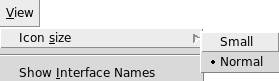
\includegraphics[width=0.4\textwidth]{./images/icon_size.png}
	\caption{\emph{Icon size menu}}
	\label{fig:icon_size}
\end{figure}

Let's take the \texttt{simple-topology.imn} example and set the icon size to
small. (Figure \ref{fig:icon_size_example})

Currently, only two sizes are available, normal and small. Otherwise, custom
icons can be used.

\begin{figure}[H]
	\centering
	\vspace{10pt}
	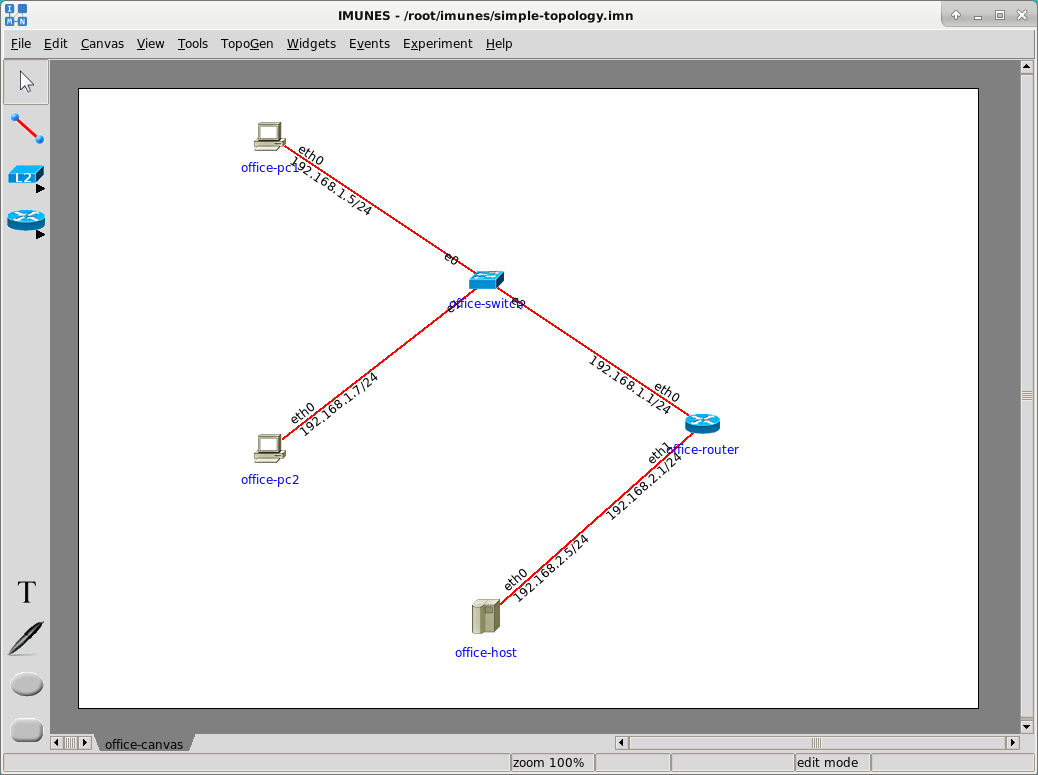
\includegraphics[width=\textwidth]{./images/icon_size_example.png}
	\caption{\emph{Icon size example}}
	\label{fig:icon_size_example}
\end{figure}
